\section{Detekcija temne snovi}

Če se ponoči zazremo v nebo, vidimo neskončno mnogo svetlih objektov, vendar je celotne vidne mase v vesolju zgolj \( 15 \% \), preostanek pa jo sestavlja temna snov, ki se deli na barionsko in nebarionsko. Bralca spomnimo, da je barionska snov sestavljena iz barionov kot so protoni in nevtroni. Trenutni rezultati eksperimentov kažejo, da je večino temne snovi nebarionske. Temno snov delimo na dva razreda -\` masivne astrofizikalne objekte v haloju (ang. \textit{massive astrophysical compact halo object} ali MACHO)~\cite{jones_introduction_2004} in hipotetične masivne delce s šibko interakcijo (ang. \textit{Weakly Interacting Massive Particles} ali WIMP)~\cite{noauthor_delec_2026}.

Kratka teorije glede WIMP-ov je povzeta iz vira~\cite{feng_dark_2010}. Njihova napovedana masa je v območju \( m_{weak} \sim 10 \, \mathrm{GeV} - \mathrm{TeV} \) in kakor pove ime interagirajo z drugimi delci preko šibke interakcije z bozonoma \( W \) in \( Z \). Po teoriji Velikega poka je bilo zgodnje vesolje gosto in vroče in delci so bili v stabilnem stanju. Ko se je vesolje kasneje ohlajalo, je temperatura \( T \) padla pod maso delca temne snovi. Boltzmannova porazdelitev nam pove verjetnost, da ima sistem določeno energijo\cite{noauthor_boltzmann_nodate}. Zaradi nje so temni delci postali zavrti in eksponentno padali \( \exp \left\{ - m_X / T  \right\} \). V naslednjem koraku se je vesolje tudi širilo, kar pomeni, da so bili delci temne snovi tako redki, da je bila njihove medsebojna anihilacija nemogoča. Število temnih delcev se tako asimptotsko približuje konstantemu številu.

WIMP-i \( X \) se torej morajo anihilirati z drugimi delci in pod predpostavko, da so te delci \( \mathrm{SM} \) del standardnega modela, potem mora obstajati interakcija \( X \, X \to \mathrm{SM} \, \mathrm{SM} \). To nam poda tri možne načine zaznave temne snovi. Če drži, da so se \( X \) anihilirali v zgodnjem vesolju, potem se morajo tudi sedaj \( X \, X \to \mathrm{SM} \, \mathrm{SM} \) in zaznamo lahko ostanke anihilacije. Temu načinu pravimo nedirektna detekcija. V trkalnikih delcev je temna snov lahko rezultat trka \( \mathrm{SM} \, \mathrm{SM} \to X \, X + \{SM\} \) in zaznamo produkte, ki nastanejo poleg temne snovi.

Zadnja vrsta detekcije, ki se tiče tega seminarja, je direktna. Temna snov se lahko sipa na normalni snovi preko interakcije

\begin{equation}
\label{eq5:1}
 X \, \mathrm{SM} \to X \, \mathrm{SM},
\end{equation}

in s tem odda svojo energijo.

Sipanje je odvisno od lokalne gostote toka \( X \) in sipalnega preseka za interakcijo. Fiksna lokalna gostota delcev \( X \) pa je odvisna od njihove mase. Eksperimentalna spremenljivka je zato izražena kot masa WIMP-a v odvisnosti od sipalnega preseka. Slednji je odvisen od interakcije WIMP-nukleon in ga delimo na spinsko odvisno in spinsko neodvisno WIMP-nukleon interakcijo~\cite{collaboration_moscab_2017}. 

Sipalni presek spinsko odvisnih interakcij je odvisen od jedrskega spinskega števila. Opisana projekta oba uporabljata na floru bazirane tekočine v mehurčni komori, saj ima jedro flora \( ^{19}F \) en nepoparjen proton, hkrati pa nima izotopov~\cite{ellis_realistic_1988}. Take tekočine imajo torej edinstveno prednost.

Mehurčne komore so dobri detektorji za direktno iskanje WIMP-ov, saj so neobčutljivi na \( \beta \) in \( \gamma \) sevanje, saj se nahajajo globoko v Zemlji\cite{collaboration_moscab_2017}. Dober detektor bo imel torej tarčo s čim večjo maso, hkrati pa bo bil občutljiv na energije pri sipanju v velikosti \( 1 - 100 \mathrm{keV} \)~\cite{amole_dark_2019}.

PICO je eden od projektov, ki preko direktne zaznave iščejo dokaze o temni snovi. Je del podzemnega laboratorija SNOLAB, ki se nahaja v Sudbury, Ontaorio v Kanadi. Od svojega nastanka 2013, ko sta se združila projekta PICASSO laboratorija SNOLAB in COUPP laboratorija Fermilab, je potekala že vrsta eksperimentov PICO-2, PICO-40 in PICO-60, kjer številka izraža količino freona v mehurčni komori. V pripravah je PICO-500\cite{noauthor_pico_nodate}. 

\begin{wrapfigure}{r}{8cm}
  \begin{center}
  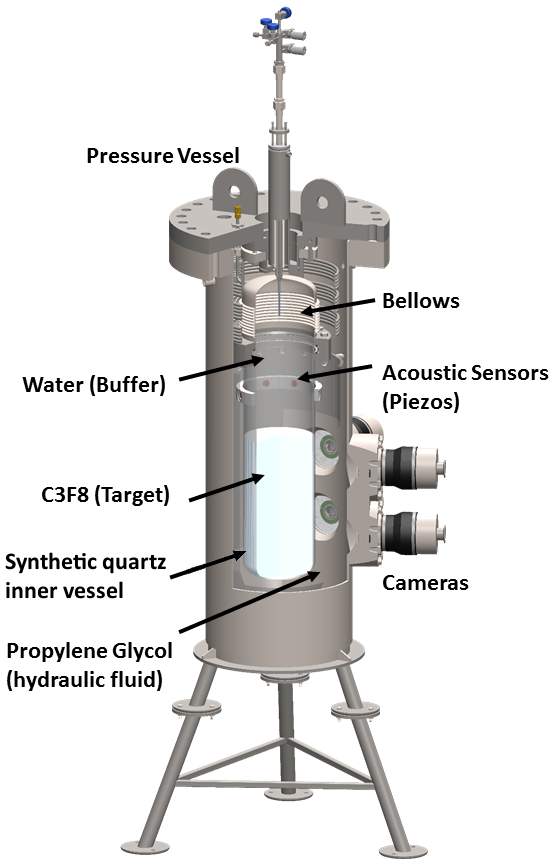
\includegraphics[width=0.25\textwidth]{./figures/PICO60Run2_IV_label}
  \end{center}
  \caption{\small Detektor PICO60~\cite{amole_dark_2019}}
\end{wrapfigure}

PICO mehurčna komora je precej drugačna od 


